\documentclass[a4paper,11pt]{article}

% ---------- Кодировка и язык ----------
\usepackage[utf8]{inputenc}
\usepackage[T2A]{fontenc}
\usepackage[english,russian]{babel}

% ---------- Геометрия страницы ----------
\usepackage[margin=2.5cm]{geometry}

% ---------- Математика ----------
\usepackage{amsmath,amssymb,amsthm,mathtools}
\usepackage{empheq}
\usepackage{bm}          % жирные символы в формулах: \bm{x}

% ---------- Оформление ----------
\usepackage{enumitem}
\usepackage{booktabs}       % красивые таблицы
\usepackage{graphicx}
\graphicspath{{figures/}}
\usepackage{xcolor}
\usepackage[colorlinks=true,linkcolor=blue,urlcolor=blue,citecolor=blue]{hyperref}
\usepackage{cleveref}       % \cref{...} для умных ссылок
\newcommand{\lean}[1]{\mbox{\path{#1}}} % имена из Lean-кода, без переносов внутри имени (пакет url)

% ---------- Теоремы и окружения ----------
\theoremstyle{plain}
\newtheorem{theorem}{Теорема}[section]
\newtheorem{lemma}[theorem]{Лемма}
\newtheorem{proposition}[theorem]{Утверждение}
\newtheorem{corollary}[theorem]{Следствие}

\theoremstyle{definition}
\newtheorem{definition}[theorem]{Определение}
\newtheorem{example}[theorem]{Пример}

\theoremstyle{remark}
\newtheorem*{remark}{Замечание}

% ---------- Полезные макросы ----------
\newcommand{\R}{\mathbb{R}}
\newcommand{\Z}{\mathbb{Z}}
\newcommand{\N}{\mathbb{N}}
\newcommand{\Q}{\mathbb{Q}}
\newcommand{\norm}[1]{\left\lVert #1 \right\rVert}
\newcommand{\abs}[1]{\left\lvert #1 \right\rvert}
\newcommand{\set}[1]{\left\{ #1 \right\}}
\newcommand{\ip}[2]{\langle #1, #2\rangle} % скалярное произведение
\newcommand{\Rpp}[1][2]{\R^{#1}_{++}} % \Rpp = R^2_{++}, \Rpp[n] = R^n_{++}
\newcommand{\Rp}[1][2]{\R^{#1}_{+}}   % \Rp = R^2_{+}, \Rp[n] = R^n_{+}

\DeclareMathOperator{\conv}{conv}
\DeclareMathOperator{\cone}{cone}
\DeclareMathOperator{\Sp}{Sp}
\DeclareMathOperator{\interior}{int}

\newcommand{\todo}[1]{\textcolor{red}{\textbf{TODO:} #1}}

\title{Наименьшее взвешенное возмущение цен\\ для слабой разрешимости}
\date{}

\begin{document}
\maketitle

\section{Введение}

Всюду $d\in\N$, $d\ge2$. Обозначения те же, что в основных заметках. Для $p,x\in\R^d$ через $p\circ x$ обозначено покоординатное произведение, через $\mathbf e:=(1,\dots,1)\in\R^d$~--- единичный вектор, через $\mathbf 1_S$~--- индикатор множества $S$. Функции $\exp$ и $\ln$ от вектора берутся покоординатно. Неравенства между векторами покоординатные.

Цены~--- наборы из $d+1$ положительных чисел, определённые с точностью до общего положительного множителя. Нормируем их по цене с номером $0$ и получаем $p\in\Rpp[d]$. Набор цен по периодам есть $P:=\set{p_t\in\Rpp[d]}_{t\in[T]}$, а $y\in\Rp[T]$~--- вектор выпусков. Каждой цене $i=0,\dots,d$ в каждом периоде $t$ сопоставлен штраф $\kappa^i_t>0$. Больший штраф означает, что цена измерена точнее.

Из основных заметок используются без доказательства следующие объекты. Вектор $y$ \textit{слабо разрешим} при ценах $P\in\Rp[d\times T]$, если в любой окрестности $P$ найдётся набор $Q\in\Rpp[d\times T]$, при котором $y$ неоклассически разрешим. Множество $S$ называется \textit{слабо достижимым спектром} при ценах $P$, если для каждого $t\in S$ существует ненулевой $\xi\in\Rp[d]$ с $\ip{\xi}{p_s-p_t}\ge0$ при всех $s\notin S$. Семейство таких множеств обозначается $\widehat{\Sp}(P)$. Индексы здесь могут пробегать любое конечное множество точек из $\Rp[d]$.

\begin{theorem}[критерий слабой разрешимости, основные заметки]\label{thm:closure}
    Вектор $y\in\Rp[T]$ слабо разрешим при ценах $P\in\Rp[d\times T]$ тогда и только тогда, когда $y\in\cone\set{\mathbf 1_S\mid S\in\widehat{\Sp}(P)}$.
\end{theorem}

\paragraph{Расстояние.}
Для нормированных цен $a,b\in\Rpp[d]$ представляющие наборы имеют вид $(\alpha a,\alpha)$ и $(\beta b,\beta)$. Положим $u_i:=\ln a^i-\ln b^i$ и $s:=\ln\alpha-\ln\beta$. Отклонение цены $i\ge1$ равно $u_i+s$, отклонение цены $0$ равно $s$. Взвешенное $\ell^\infty$-расстояние между наборами, минимизированное по $s\in\R$, даёт
\[
    d_\kappa(a,b):=\min_{s\in\R}\max\Bigl(\kappa^0\abs{s},\ \max_{i\in[d]}\kappa^i\abs{u_i+s}\Bigr).
\]
Минимум достигается, так как функция непрерывна и стремится к бесконечности. Цена $i$ известна с относительной погрешностью $\rho/\kappa^i$, где $\rho$~--- общий уровень неопределённости.

\begin{remark}[откуда берётся цена с номером $0$]
    Модель зависит только от нормированных цен. Умножение всех $d+1$ цен периода на одно число не меняет точку $p_t$. Поэтому наблюдаемы только отношения цен. Данные же состоят из $d+1$ измеренных цен $x^0,\dots,x^d$, и каждая измерена со своей ошибкой. Нормированная координата равна $\ln p^i=\ln x^i-\ln x^0$. Ошибка $\delta^i$ в цене $i\ge1$ сдвигает только координату $i$. Ошибка $\delta^0$ в цене $0$ сдвигает все координаты сразу на $-\delta^0$, то есть сдвигает точку $\ln p$ вдоль диагонали $\mathbf e$.

    Поэтому возмущение задаётся на наборе цен. Ищутся поправки $\delta^0,\dots,\delta^d$ логарифмов измеренных цен, и нормированная точка сдвигается на $u_i=\delta^i-\delta^0$. Поправки, отличающиеся общим сдвигом $\delta\mapsto\delta+c(1,\dots,1)$, дают одно и то же $u$. В обозначениях выше $\delta^0=s$ и $\delta^i=u_i+s$. Минимум по $s$ в определении $d_\kappa$ выбирает среди всех поправок, дающих данное $u$, поправку с наименьшим наибольшим взвешенным отклонением $\kappa^i\abs{\delta^i}$.

    В частности, сдвиг нормированной точки вдоль диагонали объясняется двумя способами: ошибкой в цене $0$ или одинаковой ошибкой во всех ценах $1,\dots,d$. Метрика выбирает объяснение, более дешёвое по штрафам. При $\kappa^0\to\infty$ цена $0$ считается точной, и сдвиг вдоль диагонали стоит столько же, сколько одинаковый сдвиг всех цен $1,\dots,d$.
\end{remark}

\paragraph{Задача.} Если $y$ не слабо разрешим при $P$, ищем наименьший общий уровень неопределённости, при котором найдётся набор $Q$ со слабой разрешимостью $y$:
\[
    \rho^*:=\inf\Bigl\{\rho\ge0\;\Big|\;\exists Q\in\Rpp[d\times T]:\ d_{\kappa_t}(q_t,p_t)\le\rho\ \ \forall t\in[T],\ y\text{ слабо разрешим при }Q\Bigr\}.
\]

\paragraph{Результаты.} Положим $v^i_t:=1/\kappa^i_t+1/\kappa^0_t$.
\begin{enumerate}[label=(\roman*)]
    \item Шар $\set{d_\kappa(\cdot,p)\le\rho}$ в логарифмических координатах есть зонотоп: коробка, сдвинутая вдоль диагонали (лемма~\ref{lem:shape}).
    \item Задача сводится к одному запросу к оракулу в угловых точках $p_t\circ e^{\mp\rho v_t}$ и к одному параметру на период на логарифмически линейном пути $\theta\mapsto p_t\circ e^{\theta v_t}$, $\abs{\theta}\le\rho$ (теорема~\ref{thm:corners}). Относительные цены при этом меняются, причём дешевле двигаются цены с меньшим штрафом.
    \item Наименьший уровень $\rho^*$ достигается и является точкой излома (теорема~\ref{thm:least}).
    \item Бисекция с безопасным рациональным округлением находит $\rho^*$ с точностью $\varepsilon$ за $O(\log(1/\varepsilon))$ обращений к оракулу при любых штрафах. Если штрафы равны, то $v^i_t=c$ для всех $i,t$ и угловые точки равны $p_te^{\mp\rho c}$. Тогда точки излома рациональны как функции от $z=e^{2\rho c}$, и $\rho^*$ находится точным поиском за $O(d\log(T+d))$ обращений. Оракул проверяет слабую разрешимость с двусторонними границами. При $d=2$ оракул есть одна задача линейного программирования о потоке (\texttt{poly-hardness/}), и алгоритм полиномиален. При $d\ge3$ оракул NP-труден (\texttt{np-hardness/}), на практике используется генерация столбцов.
\end{enumerate}

\section{Метрика}

Пусть $a,b\in\Rpp[d]$, $u_i:=\ln a^i-\ln b^i$ и $\kappa^0,\dots,\kappa^d>0$.

\begin{lemma}[форма шара]\label{lem:shape}
    Пусть $\rho\ge0$. Тогда $d_\kappa(a,b)\le\rho$ тогда и только тогда, когда существует $s\in\R$ с
    \[
        \kappa^0\abs{s}\le\rho,\qquad\kappa^i\abs{u_i+s}\le\rho\ \ (i\in[d]).
    \]
    То есть шар в координатах $u$ есть множество $\prod_i[-\rho/\kappa^i,\rho/\kappa^i]+\set{s\mathbf e\mid\abs{s}\le\rho/\kappa^0}$. Это зонотоп.
\end{lemma}

\begin{proof}
    Минимум по $s$ достигается, поэтому $d_\kappa(a,b)\le\rho$ равносильно существованию $s$ со значением целевой функции не больше $\rho$. Это и есть система неравенств.
\end{proof}

\lean{wdist_le_iff}.

\begin{corollary}\label{cor:ball}
    Шар $\set{q\in\Rpp[d]\mid d_\kappa(q,p)\le\rho}$ лежит в коробке $\abs{\ln q^i-\ln p^i}\le\rho v^i$, то есть $p\circ e^{-\rho v}\le q\le p\circ e^{\rho v}$. Он содержит угловые точки $p\circ e^{\pm\rho v}$ и путь $\set{p\circ e^{\theta v}\mid\abs{\theta}\le\rho}$.
\end{corollary}

\begin{proof}
    Пусть $u=\ln q-\ln p$ и $s$ из леммы~\ref{lem:shape}. Тогда $\abs{u_i}\le\abs{u_i+s}+\abs{s}\le\rho/\kappa^i+\rho/\kappa^0$. Для точки пути $u=\theta v$. Возьмём $s:=-\theta/\kappa^0$. Тогда $\kappa^0\abs{s}=\abs{\theta}\le\rho$ и $u_i+s=\theta/\kappa^i$, откуда $\kappa^i\abs{u_i+s}=\abs{\theta}\le\rho$. При $\theta=\pm\rho$ получаем угловые точки.
\end{proof}

\lean{mem_wbox_of_wdist}, \lean{wdist_wpath_le}.

\paragraph{Частный случай.} При $\kappa^0\to\infty$ шар есть коробка $\prod_i[-\rho/\kappa^i,\rho/\kappa^i]$: цена с номером $0$ фиксирована.

\section{Сведение к углам}

Пусть $W=\set{w_r}_{r\in R}\subset\Rpp[d]$~--- конечный набор точек. Для $S\subset R$ положим
\[
    K_S:=\conv\set{w_r\mid r\notin S}+\Rp[d],\qquad K_R:=\varnothing.
\]
Множество $K_S$ выпукло, замкнуто, и $K_S+\Rp[d]\subset K_S$. Для $S\ne R$ оно имеет непустую внутренность и лежит в $\Rpp[d]$.

\begin{lemma}[достижимость и внутренность]\label{lem:interior}
    Пусть $S\subset R$, $t\in S$. Ненулевой $\xi\in\Rp[d]$ с $\ip{\xi}{w_s-w_t}\ge0$ при всех $s\notin S$ существует тогда и только тогда, когда $w_t\notin\interior K_S$. Поэтому $S\in\widehat{\Sp}(W)$ тогда и только тогда, когда ни одна точка $w_t$, $t\in S$, не лежит в $\interior K_S$.
\end{lemma}

\begin{proof}
    Для $\xi\ge0$ условие $\ip{\xi}{w_s-w_t}\ge0$ при $s\notin S$ равносильно $\ip{\xi}{z-w_t}\ge0$ на $K_S$. Если $w_t\in\interior K_S$ и $\xi\ne0$, то точка $w_t-\varepsilon\xi$ лежит в $K_S$ при малом $\varepsilon>0$, и значение равно $-\varepsilon\norm{\xi}^2<0$. Значит, $\xi$ не подходит. Обратно, пусть $w_t\notin\interior K_S$. Если $K_S=\varnothing$, подходит любой ненулевой $\xi\ge0$. Иначе по теореме отделимости точки от открытого выпуклого множества $\interior K_S$ найдётся ненулевая линейная функция $\ip{\xi}{\cdot}$ с $\ip{\xi}{z-w_t}\ge0$ на $\interior K_S$, а значит и на $K_S=\overline{\interior K_S}$. Из $K_S+\Rp[d]\subset K_S$ получаем $\xi\ge0$.
\end{proof}

\begin{lemma}[выход вдоль пути]\label{lem:ray}
    Пусть $z:\R\to\Rpp[d]$~--- непрерывный путь, все координаты которого строго возрастают, $z(\theta)\to0$ при $\theta\to-\infty$ и $z(\theta)\to\infty$ при $\theta\to+\infty$ покоординатно. Пусть $S\ne R$ и $\gamma:=\min\set{\theta\mid z(\theta)\in K_S}$. Тогда
    \[
        \set{\theta\mid z(\theta)\notin\interior K_S}=(-\infty,\gamma],\qquad\set{\theta\mid z(\theta)\notin K_S}=(-\infty,\gamma).
    \]
    Для $S=R$ положим $\gamma:=+\infty$, и оба множества равны $\R$.
\end{lemma}

\begin{proof}
    Множество $\set{\theta\mid z(\theta)\in K_S}$ замкнуто. Оно непусто, так как $K_S\supset w+\Rp[d]$ при некотором $w$ и $z(\theta)\ge w$ при больших $\theta$. Оно ограничено снизу, так как $K_S\subset\set{x\mid x\ge\min_rw_r}$ и $z(\theta)\to0$. Поэтому $\gamma$ существует. Если $z(\theta)\in K_S$ и $\theta'>\theta$, то $z(\theta')=z(\theta)+(z(\theta')-z(\theta))$ и $z(\theta')-z(\theta)\in\interior\Rp[d]$, поэтому $z(\theta')\in\interior K_S$. Отсюда $\set{\theta\mid z(\theta)\in K_S}=[\gamma,\infty)$ и $(\gamma,\infty)\subset\set{\theta\mid z(\theta)\in\interior K_S}$. Точка $z(\gamma)$ не лежит во внутренности, так как $z(\gamma-\varepsilon)\notin K_S$ при $\varepsilon>0$.
\end{proof}

Для пути $z(\theta)=p\circ e^{\theta v}$, $v>0$, условия леммы выполнены. Для доказательства теоремы~\ref{thm:corners} в Lean (\lean{path_of_corners}) достаточно непрерывности пути, значений в концах и неотрицательности. В тексте путь оставлен монотонным для ясности.

Пусть $a_t:=p_t\circ e^{-\rho v_t}$, $b_t:=p_t\circ e^{\rho v_t}$ и $W:=(a,b)$ с индексами $R=\set{a_t,b_t}_{t\in[T]}$. Для $w:=\sum_km_k\mathbf 1_{S_k}$ значение $w(r)$ есть $\sum_km_k\mathbf 1_{S_k}(r)$.

\begin{theorem}[углы]\label{thm:corners}
    Пусть $d\ge2$, $y\in\Rp[T]$, $\rho\ge0$. Равносильны:
    \begin{enumerate}[label=(\Alph*)]
        \item существует $Q\in\Rpp[d\times T]$ с $d_{\kappa_t}(q_t,p_t)\le\rho$ при всех $t$, при котором $y$ слабо разрешим,
        \item существуют $\theta_t\in[-\rho,\rho]$, при которых $y$ слабо разрешим при ценах $(p_t\circ e^{\theta_tv_t})_{t\in[T]}$,
        \item существует $w\in\cone\set{\mathbf 1_S\mid S\in\widehat{\Sp}(W)}$ с $w(a_t)\ge y_t\ge w(b_t)$ при всех $t\in[T]$.
    \end{enumerate}
\end{theorem}

\lean{wfeasible_iff_corners}, \lean{wfeasible_iff_path}.

\begin{proof}
    (B)$\Rightarrow$(A). Точка пути лежит в шаре по следствию~\ref{cor:ball}: сдвиг $s=-\theta_t/\kappa^0_t$.

    (A)$\Rightarrow$(C). По теореме~\ref{thm:closure} $y=\sum_km_k\mathbf 1_{S_k}$ с $m_k>0$ и $S_k\in\widehat{\Sp}(Q)$. Положим $K_k:=K_{S_k}(Q)$. По следствию~\ref{cor:ball} $a_t\le q_t\le b_t$. Определим $S'_k\subset R$:
    \[
        a_t\in S'_k\iff a_t\notin\interior K_k,\qquad b_t\in S'_k\iff b_t\notin K_k.
    \]
    \emph{Шаг 1: $S'_k\in\widehat{\Sp}(W)$.} Если $a_t\notin S'_k$, то $a_t\in\interior K_k$. Если $b_t\notin S'_k$, то $b_t\in K_k$. Поэтому $K_{S'_k}(W)\subset K_k$, и $\interior K_{S'_k}(W)\subset\interior K_k$. Для $a_t\in S'_k$ имеем $a_t\notin\interior K_k\supset\interior K_{S'_k}(W)$. Для $b_t\in S'_k$ имеем $b_t\notin K_k\supset K_{S'_k}(W)$. По лемме~\ref{lem:interior} $S'_k\in\widehat{\Sp}(W)$.

    \emph{Шаг 2: границы.} Пусть $t\in S_k$. Тогда $q_t\notin\interior K_k$. Если бы $a_t\in\interior K_k$, то $q_t\in a_t+\Rp[d]\subset\interior K_k$. Значит, $a_t\in S'_k$. Пусть $b_t\in S'_k$. Тогда $b_t\notin K_k$, и $q_t\notin K_k$, так как $q_t\le b_t$ и $K_k+\Rp[d]\subset K_k$. Значит, $t\in S_k$. Для $w:=\sum_km_k\mathbf 1_{S'_k}$ получаем $w(a_t)\ge y_t\ge w(b_t)$.

    (C)$\Rightarrow$(B). Пусть $w=\sum_km_k\mathbf 1_{S'_k}$, $m_k>0$, $S'_k\in\widehat{\Sp}(W)$, и $K_k:=K_{S'_k}(W)$. Пусть $z_t(\theta):=p_t\circ e^{\theta v_t}$ и $\gamma_{k,t}\in(-\infty,\infty]$~--- число из леммы~\ref{lem:ray} для $K_k$ и пути $z_t$. Положим
    \[
        \mathrm{hi}_t(\theta):=\sum_km_k\mathbf 1[\theta\le\gamma_{k,t}],\qquad\mathrm{lo}_t(\theta):=\sum_km_k\mathbf 1[\theta<\gamma_{k,t}].
    \]
    Если $a_t=z_t(-\rho)\in S'_k$, то по леммам~\ref{lem:interior} и~\ref{lem:ray} $-\rho\le\gamma_{k,t}$. Если $b_t=z_t(\rho)\notin S'_k$, то $b_t\in K_k$ и $\gamma_{k,t}\le\rho$. Поэтому
    \[
        \mathrm{hi}_t(-\rho)\ge w(a_t)\ge y_t\ge w(b_t)\ge\mathrm{lo}_t(\rho).
    \]
    Функция $\mathrm{hi}_t$ не возрастает, и множество $\set{\theta\mid\mathrm{hi}_t(\theta)\ge y_t}$ замкнуто. Положим $\theta_t:=\max\set{\theta\in[-\rho,\rho]\mid\mathrm{hi}_t(\theta)\ge y_t}$. Это множество содержит $-\rho$, поэтому $\theta_t$ определено и $\mathrm{hi}_t(\theta_t)\ge y_t$. Покажем $\mathrm{lo}_t(\theta_t)\le y_t$. Если $\theta_t=\rho$, это доказано выше. Иначе $\mathrm{hi}_t(\theta)<y_t$ при $\theta\in(\theta_t,\rho]$, и $\mathrm{lo}_t(\theta_t)=\lim_{\theta\downarrow\theta_t}\mathrm{hi}_t(\theta)\le y_t$.

    Положим $q_t:=z_t(\theta_t)$ и $A_k:=\set{t\mid\theta_t<\gamma_{k,t}}$, $B_k:=\set{t\mid\theta_t\le\gamma_{k,t}}$. Тогда $\mathrm{lo}=\sum_km_k\mathbf 1_{A_k}\le y\le\sum_km_k\mathbf 1_{B_k}=\mathrm{hi}$ покоординатно. По лемме~\ref{lem:cube} ниже $y=\sum_j\mu_j\mathbf 1_{C_j}$, $\mu_j>0$, где каждое $C_j$ удовлетворяет $A_k\subset C_j\subset B_k$ при некотором $k$. Осталось проверить $C_j\in\widehat{\Sp}(Q)$, и тогда $y$ слабо разрешим при $Q$ по теореме~\ref{thm:closure}.

    Пусть $A_k\subset C\subset B_k$ и $s\notin C$. Тогда $s\notin A_k$, то есть $\theta_s\ge\gamma_{k,s}$, и $q_s\in K_k$ по лемме~\ref{lem:ray}. Поэтому $K_C(Q)\subset K_k$. Для $t\in C\subset B_k$ имеем $\theta_t\le\gamma_{k,t}$, и $q_t\notin\interior K_k\supset\interior K_C(Q)$ по лемме~\ref{lem:ray}. По лемме~\ref{lem:interior} $C\in\widehat{\Sp}(Q)$.
\end{proof}

\begin{lemma}[куб]\label{lem:cube}
    Пусть $m_k>0$, $A_k\subset B_k\subset[T]$ при $k\in[n]$, и $\sum_km_k\mathbf 1_{A_k}\le y\le\sum_km_k\mathbf 1_{B_k}$. Тогда $y=\sum_j\mu_j\mathbf 1_{C_j}$ с $\mu_j>0$, причём для каждого $j$ найдётся $k$ с $A_k\subset C_j\subset B_k$.
\end{lemma}

\begin{proof}
    Разместим на $[0,M)$, $M:=\sum_km_k$, последовательные интервалы $I_k$ длины $m_k$ и обозначим через $k(x)$ номер интервала, содержащего $x$. Для $t\in[T]$ положим $E_t:=\bigcup_{k:\,t\in B_k\setminus A_k}I_k$ и $\ell_t:=\sum_km_k\mathbf 1_{A_k}(t)$. Тогда $\abs{E_t}=\sum_km_k\bigl(\mathbf 1_{B_k}(t)-\mathbf 1_{A_k}(t)\bigr)\ge y_t-\ell_t\ge0$. Возьмём начальный отрезок $F_t:=E_t\cap[0,x_t)$ меры $y_t-\ell_t$ и положим $C(x):=A_{k(x)}\cup\set{t\mid x\in F_t}$. Тогда $A_{k(x)}\subset C(x)\subset B_{k(x)}$, мера множества $\set{x\mid t\in C(x)}$ равна $\ell_t+(y_t-\ell_t)=y_t$, а $C(x)$ кусочно постоянна с конечным числом интервалов постоянства.
\end{proof}

Лемму можно получить и из \lean{PolyHardness.cube_mem_span} (\texttt{poly-hardness/}).

\begin{remark}[метрика выбирает только коробку]
    В доказательстве теоремы~\ref{thm:corners} от шара используются два свойства: он лежит в коробке с угловыми точками $p_t\circ e^{\mp\rho v_t}$ и содержит эти точки вместе с монотонным путём между ними. Поэтому для любой области возмущений с этими свойствами задача равносильна задаче о коробке, и все дальнейшие результаты (точки излома, наименьший радиус, сложность, профили) зависят только от размеров коробок. Метрика $d_\kappa$ лишь задаёт эти размеры. Если область не содержит угловых точек своей описанной коробки, сведение к коробке теряется, и задача становится существенно $dT$-мерной.
\end{remark}

\section{Точки излома}

Семейство $\widehat{\Sp}$ не меняется при общем положительном масштабе точек, а также при положительном масштабе каждой координаты: $\widehat{\Sp}(D W)=\widehat{\Sp}(W)$ для диагональной матрицы $D$ с положительными элементами. Здесь $\xi$ заменяется на $D^{-1}\xi\ge0$.

\paragraph{Однородные векторы.} Точке $w_r$ сопоставим вектор $(w_r,1)\in\R^{d+1}$ и добавим векторы $(e_i,0)$, $i\in[d]$. Для линейной функции $\eta=(\xi,\eta_0)$ на $\R^{d+1}$ положим $\eta(w,1)=\ip{\xi}{w}+\eta_0$.

\begin{lemma}[слабая достижимость как условие на знаки]\label{lem:signs}
    Индекс $t\in S$ имеет слабого свидетеля тогда и только тогда, когда существует ненулевая линейная функция $\eta$ на $\R^{d+1}$ с $\eta(w_t,1)=0$, $\eta(w_s,1)\ge0$ при $s\notin S$ и $\eta(e_i,0)\ge0$ при $i\in[d]$.
\end{lemma}

\lean{witness_iff_homogeneous}.

\begin{proof}
    По свидетелю $\xi$ положим $\eta:=(\xi,-\ip{\xi}{w_t})$. Тогда $\eta(w_s,1)=\ip{\xi}{w_s-w_t}$, $\eta(e_i,0)=\xi^i$, и $\eta\ne0$, так как $\xi\ne0$. Обратно, из $\eta(w_t,1)=0$ следует $\eta_0=-\ip{\xi}{w_t}$, и $\eta\ne0$ равносильно $\xi\ne0$.
\end{proof}

Знаковым вектором функции $\eta$ называется набор знаков $\eta(v_j)$ по всем векторам $v_j$ конфигурации.

\begin{lemma}[локальное постоянство]\label{lem:local}
    Пусть $I\subset\R$~--- интервал, $v_j:I\to\R^{d+1}$, $j\in J$,~--- конечный набор непрерывных функций, векторы $v_j(\rho)$ при каждом $\rho$ порождают $\R^{d+1}$. Пусть $\rho_0\in I$ и каждый определитель $\det(v_j)_{j\in B}$, $B\subset J$, $\abs{B}=d+1$, либо тождественно равен нулю на $I$, либо не равен нулю в $\rho_0$. Тогда всякий знаковый вектор ненулевой функции при $\rho_0$ реализуется ненулевой функцией при всех $\rho$ из некоторой окрестности $\rho_0$.
\end{lemma}

\lean{eventually_exists_sign_eq}.

\begin{proof}
    Определители, не равные тождественно нулю, не равны нулю в $\rho_0$ и по непрерывности в некоторой окрестности $N\ni\rho_0$. Поэтому в $N$ каждый определитель либо равен нулю тождественно, либо не равен нулю ни в одной точке.

    \emph{Независимость не зависит от $\rho\in N$.} Пусть $Z'\subset J$ независимо при $\rho_1\in N$. Так как $v_j(\rho_1)$ порождают $\R^{d+1}$, достроим $Z'$ до базиса $B\subset J$. Тогда $\det_B(\rho_1)\ne0$, значит, определитель не равен нулю тождественно, и $\det_B(\rho)\ne0$ при всех $\rho\in N$. Поэтому $Z'$ независимо при всех $\rho\in N$. В частности, ранг любого $Z\subset J$ постоянен на $N$.

    Пусть $\eta$~--- ненулевая функция при $\rho_0$, $Z:=\set{j\mid\eta(v_j(\rho_0))=0}$ и $r:=\operatorname{rank}Z$. Выберем независимое $Z_0\subset Z$ с $\abs{Z_0}=r$. Оно независимо и при всех $\rho\in N$, и порождает $\operatorname{span}\set{v_j(\rho)}_{j\in Z}$, так как ранг $Z$ равен $r$. Достроим $Z_0$ набором $C\subset J$, $\abs{C}=d+1-r$, до базиса. Он является базисом при всех $\rho\in N$. Определим $\eta_\rho$ условиями
    \[
        \eta_\rho(v_j(\rho))=0\ (j\in Z_0),\qquad\eta_\rho(v_c(\rho))=\eta(v_c(\rho_0))\ (c\in C).
    \]
    Коэффициенты $\eta_\rho$ непрерывны по $\rho$, и $\eta_{\rho_0}=\eta$. Для $j\in Z$ вектор $v_j(\rho)$ лежит в $\operatorname{span}Z_0(\rho)$, поэтому $\eta_\rho(v_j(\rho))=0$ при всех $\rho\in N$. Для $j\notin Z$ значение $\eta_\rho(v_j(\rho))$ непрерывно и в $\rho_0$ отлично от нуля, поэтому знак сохраняется вблизи $\rho_0$. Индексов конечное число, поэтому окрестность можно выбрать общей. Функция $\eta_\rho$ ненулевая, так как конфигурация порождает $\R^{d+1}$ и $\eta_\rho(v_j(\rho))\ne0$ при некотором $j$ (знаковый вектор $\eta$ не нулевой).
\end{proof}

\begin{corollary}\label{cor:local}
    Пусть $W(\rho)$~--- конечное семейство точек $w_r(\rho)\in\Rpp[d]$, непрерывно зависящих от $\rho$. Пусть в точке $\rho_0$ каждый определитель конфигурации $(w_r(\rho),1)$, $(e_i,0)$ либо равен нулю тождественно, либо не равен нулю при $\rho_0$. Тогда $\widehat{\Sp}(W(\rho))\supseteq\widehat{\Sp}(W(\rho_0))$ для всех $\rho$ из некоторой окрестности $\rho_0$.
\end{corollary}

\lean{eventually_isWeakReachable_of}.

\begin{proof}
    Пусть $S\in\widehat{\Sp}(W(\rho_0))$ и $t\in S$. По лемме~\ref{lem:signs} функция $\eta$ для пары $(S,t)$ задаёт знаковый вектор с нулём на $v_t$ и неотрицательными знаками на $v_s$, $s\notin S$, и на $(e_i,0)$. По лемме~\ref{lem:local} такой вектор реализуется ненулевой функцией при всех $\rho$ вблизи $\rho_0$. Пар $(S,t)$ конечное число.
\end{proof}

\paragraph{Точки излома.} Рассмотрим конфигурацию из $2T+d$ векторов $(a_t,1)$, $(b_t,1)$, $(e_i,0)$. \textit{Точками излома} назовём значения $\rho>0$, при которых обращается в нуль определитель $(d+1)$-подмножества этой конфигурации, не равный нулю тождественно. Элементы строк $(a_t,1)$ и $(b_t,1)$ суть $p^i_te^{\mp\rho v^i_t}$ и $1$. Поэтому определитель есть конечная сумма $\sum_rC_re^{\rho\lambda_r}$ с вещественными $C_r,\lambda_r$. Это аналитическая функция от $\rho$, и если она не равна нулю тождественно, то её нули дискретны. Значит, на любом отрезке точек излома конечное число. При разных штрафах они вообще говоря не рациональны.

\paragraph{Равные штрафы.} Пусть $v^i_t=c$ для всех $i,t$. Тогда $W=(e^{-\rho c}P,e^{\rho c}P)$, и по однородности семейство $\widehat{\Sp}(W)$ совпадает с семейством для $(P,zP)$, $z:=e^{2\rho c}$. Рассмотрим $(d+1)$-подмножество $B$ конфигурации $(P,zP)$ с $\alpha$ строками вида $(p_t,1)$, $\beta$ строками вида $(zp_s,1)$ и остальными вида $(e_i,0)$. Разделим строки второго вида на $z>0$. Они станут $(p_s,1/z)$, и определитель домножится на $z^{-\beta}$. Первые $d$ столбцов полученной матрицы $X$ не зависят от $z$, а последний столбец равен $\mathbf u+z^{-1}\mathbf v$, где $\mathbf u$ и $\mathbf v$~--- индикаторы строк первого и второго вида. Определитель линеен по последнему столбцу, поэтому
\[
    \det{}_B(z)=z^{\beta}\bigl(D_0+z^{-1}D_1\bigr)=z^{\beta-1}(D_0z+D_1),\qquad D_0=\det[X\mid\mathbf u],\ D_1=\det[X\mid\mathbf v].
\]
Если $D_0=0$, то определитель равен нулю тождественно или не обращается в нуль при $z>0$. Если $D_0\ne0$, то у него единственный корень $z=-D_1/D_0$. Если $P$ рационально, то $D_0,D_1\in\Q$. Поэтому точки излома по $z$ рациональны. Подмножеств $B$ не более $\binom{2T+d}{d+1}$, поэтому точек излома $N=O\bigl((2T+d)^{d+1}\bigr)$.

\section{Теорема о наименьшем радиусе}

Пусть $F:=\set{\rho\ge0\mid\text{выполнено (A)}}$.

\begin{theorem}[наименьший радиус]\label{thm:least}
    Если $F\ne\varnothing$, то $F=[\rho^*,\infty)$. При этом $\rho^*=0$ или $\rho^*$ является точкой излома.
\end{theorem}

\lean{least_wradius_breakpoint}.

\begin{proof}
    \emph{Монотонность.} Шары вложены друг в друга, поэтому из $\rho\in F$ следует $[\rho,\infty)\subset F$.

    \emph{Замкнутость.} Пусть $\rho_n\in F$, $\rho_n\downarrow\rho$. По теореме~\ref{thm:corners} найдутся $\theta^{(n)}\in[-\rho_n,\rho_n]^T$, при которых $y$ слабо разрешим при ценах $(p_t\circ e^{\theta^{(n)}_tv_t})_t$. Переходя к подпоследовательности, считаем $\theta^{(n)}\to\theta\in[-\rho,\rho]^T$. Слабая разрешимость замкнута. Действительно, любая окрестность $U$ набора цен в пределе содержит набор для $\theta^{(n)}$ при большом $n$ вместе с некоторой окрестностью, и в ней по определению есть набор, при котором $y$ разрешим. Значит, $y$ слабо разрешим при ценах для $\theta$, и $\rho\in F$ по теореме~\ref{thm:corners}.

    \emph{Точка излома.} Пусть $\rho^*>0$ и $\rho^*$ не является точкой излома. Тогда каждый определитель конфигурации углов либо равен нулю тождественно, либо не равен нулю при $\rho^*$. По теореме~\ref{thm:corners} выполнено (C) при $\rho^*$. По следствию~\ref{cor:local} при $\rho<\rho^*$ достаточно близком к $\rho^*$ семейство $\widehat{\Sp}(W(\rho))$ содержит $\widehat{\Sp}(W(\rho^*))$. Индексы $a_t,b_t$ и значения $y_t$ те же, поэтому $w$ из (C) при $\rho^*$ годится и при $\rho$. По теореме~\ref{thm:corners} $\rho\in F$, что противоречит определению $\rho^*$.
\end{proof}

\begin{corollary}\label{cor:gap}
    На каждом интервале между соседними точками излома (а также на $(0,\rho_1)$ и $(\rho_N,\infty)$) допустимость постоянна.
\end{corollary}

\section{Профиль поправок}\label{sec:profile}

Число $\rho^*$ задаёт только наибольшую необходимую поправку. Решение, построенное в доказательстве теоремы~\ref{thm:corners}, сдвигает многие периоды до предела $\rho^*$, хотя им это не нужно. Чтобы выделить действительно необходимые поправки, дадим каждому периоду свой радиус.

\paragraph{Радиусы по периодам.} Для $r\in\R^T$ положим $r\in\mathcal R$, если найдётся $Q$ с $d_{\kappa_t}(q_t,p_t)\le r_t$ при всех $t$, при котором $y$ слабо разрешим. Свой радиус $r_t$ равносилен общему радиусу $\rho$ при штрафах $\kappa_t\rho/r_t$. Поэтому теорема~\ref{thm:corners} переносится: $r\in\mathcal R$ тогда и только тогда, когда выполнено условие на углы $p_t\circ e^{\mp r_tv_t}$, и тогда и только тогда, когда найдутся $\theta$ с $\abs{\theta_t}\le r_t$ и слабой разрешимостью в точках $p_t\circ e^{\theta_tv_t}$. Множество $\mathcal R$ замкнуто вверх и замкнуто. Под каждым $r\in\mathcal R$ лежит минимальный по Парето элемент $\mathcal R$.

\paragraph{Наименьшего элемента нет.} Множество $\mathcal R$ не замкнуто относительно покоординатного минимума. Причина простая: часто можно исправить либо один период, либо другой, но не обойтись без обоих. Пример при $d=2$, $T=3$: $p_1=(2,3)$, $p_2=(9/5,9/5)$, $p_3=(5/2,9/2)$, $y=(4,4,5)$, штрафы $\kappa_1=(1,3)$, $\kappa_2=(2,2)$, $\kappa_3=(3,1)$, $\kappa^0=(4,1,2)$. По ответам оракула векторы $r=(0,0,0.394)$ и $r'=(0.073,0.163,0.159)$ лежат в $\mathcal R$, а их минимум $(0,0,0.159)$ не лежит. В случайных примерах при $d=2$ и $d=3$ минимум двух допустимых векторов недопустим в подавляющем большинстве пар. Поэтому у $\mathcal R$ нет наименьшего элемента, и канонический выбор требует порядка.

\paragraph{Лексикографический минимум.} \textit{Профилем} назовём $r\in\mathcal R$, у которого убывающая перестановка лексикографически наименьшая. Он минимален по Парето. Профиль находится по стадиям. Пусть годы $F$ зафиксированы с радиусами $r_F$, а годы $G$ свободны.
\begin{enumerate}
    \item Наименьший общий радиус $\rho(F)$ свободных лет при зафиксированных $r_F$ находится бисекцией. Это следующее значение убывающей перестановки профиля: меньше нельзя, а все свободные годы на уровне $\rho(F)$ допустимы.
    \item Нужно наименьшее по числу элементов множество $B\subset G$, при котором все годы $G\setminus B$ одновременно опускаются ниже $\rho(F)$. Всякое такое $B$ содержит множество $B_0$ лет, которые нельзя опустить поодиночке. Если $G\setminus B_0$ опускается одновременно, то $B=B_0$. Иначе перебираются надмножества $B_0$ по возрастанию размера, а при нескольких минимальных $B$ процедура ветвится и выбирает лексикографически наименьший итог.
    \item Годы $B$ фиксируются на уровне $\rho(F)$, и шаг повторяется.
\end{enumerate}
Процедура точна с точностью бисекции при любых данных. Без ветвления она делает $O(T^2\log(1/\varepsilon))$ обращений к оракулу. С ветвлением число обращений в худшем случае экспоненциально по $T$. В 427 случайных примерах ветвление понадобилось один раз, и там все три радиуса совпали с точностью $4\cdot10^{-6}$, то есть это эффект допуска бисекции.

\paragraph{Пример.} Данные США со штрафами из примера ниже. Профиль имеет 24 стадии и найден за 1015 обращений, 188 с, без ветвления. На первой стадии зафиксированы 2008 и 2020 годы с $r_t=\rho^*=0.0581$. Двигаются все 26 периодов. Наименьший радиус $0.0027$ у 2005 года.

\begin{figure}[ht]
    \centering
    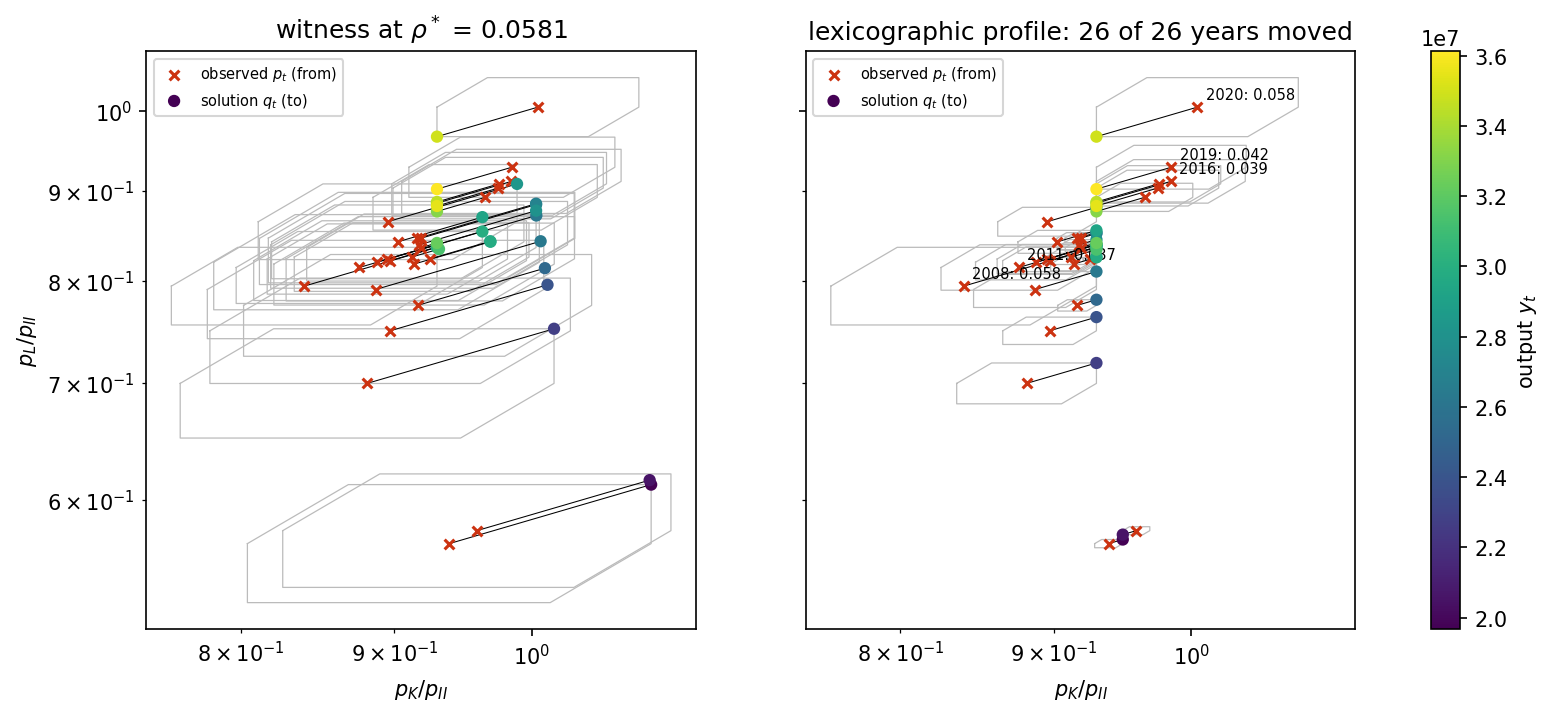
\includegraphics[width=\textwidth]{example_profile.png}
    \caption{Слева~--- решение из доказательства теоремы~\ref{thm:corners} при $\rho^*$, справа~--- профиль. Крестики~--- наблюдения, точки~--- решения.}
\end{figure}

В профиле решения почти всех периодов легли на вертикальную прямую $p_K/p_{II}\approx0.93$. Объяснение такое. Если у точек совпадает первая координата, то для любого множества $S$ подходит свидетель $\xi=e_1$: $\ip{\xi}{p_s-p_t}=0$. Тогда слабо достижимо любое множество, и любой $y$ слабо разрешим. Цена капитала имеет наименьший штраф, поэтому выравнивание отношения $p_K/p_{II}$ по годам есть дешёвый способ сделать $y$ слабо разрешимым. Это наблюдение на одном примере, а не теорема.

\todo{Проверить, всегда ли профиль при одном наименьшем штрафе сводит точки к гиперплоскости $p_i=\mathrm{const}$ для цены $i$ с наименьшим штрафом, и обобщить объяснение.}

\paragraph{Профиль по парам «цена $\times$ период».} Та же процедура применима к более мелким единицам. Без штрафов дадим каждой паре $(t,i)$ свою полуширину $a_{t,i}$ коробки: $p^i_te^{-a_{t,i}}\le q^i_t\le p^i_te^{a_{t,i}}$. Это прямо задача о коробке, без метрики. Профилем назовём лексикографический минимум убывающей перестановки вектора $(a_{t,i})$ из $\R^{dT}$. Первая стадия даёт общую полуширину $\rho^*$. Затем фиксируются пары, на стенку которых село решение, и процедура повторяется для остальных. Пара, которой решение не касается, заведомо не блокирующая, поэтому поодиночке проверяются только касающиеся пары. Поиск надмножеств при совместной проверке идёт по всем свободным парам, и ответ точен с точностью бисекции.

На данных США $\rho^*=0.0897$, профиль имеет 33 стадии и найден за 976 обращений, 181 с, без ветвления. 16 пар из 52 не двигаются. Наибольшие поправки у пары (2008, K) и (2020, K), обе $0.0897$. В большинстве лет двигается только одна цена, чаще всего $p_K/p_{II}$. Решения снова почти выстраиваются на вертикальной прямой $p_K/p_{II}\approx0.92$--$0.93$.

\begin{figure}[ht]
    \centering
    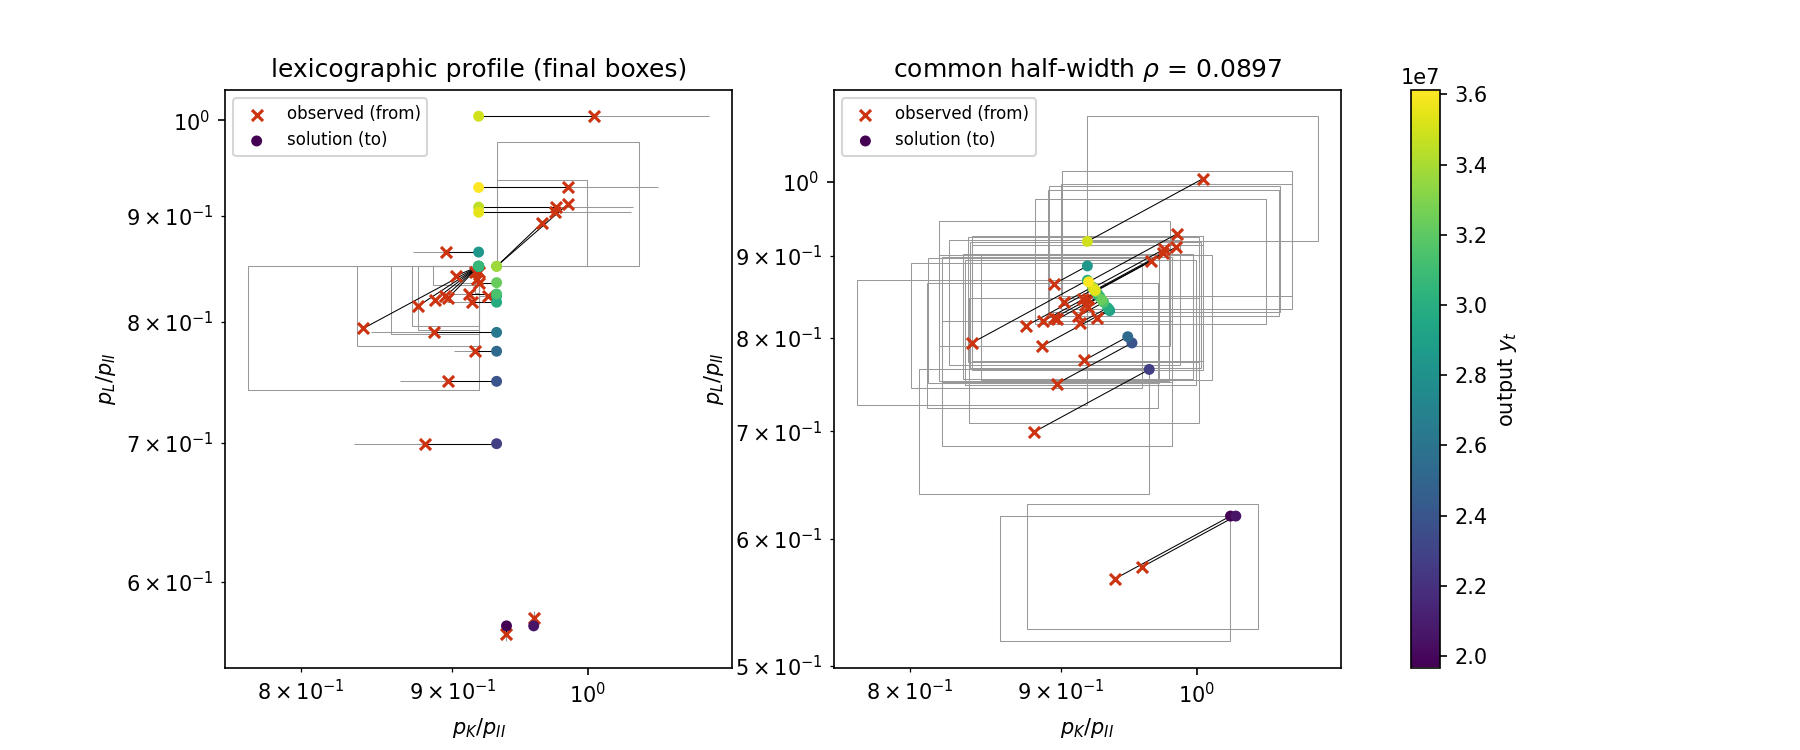
\includegraphics[width=\textwidth]{example_pairs.png}
    \caption{Слева~--- профиль по парам (итоговые коробки своих размеров), справа~--- решение при общей полуширине $\rho^*$. Крестики~--- наблюдения, точки~--- решения.}
\end{figure}

\section{Алгоритм}

\paragraph{Оракул.} Для набора точек $W$ с индексами $R$ и границ $\mathrm{lo},\mathrm{hi}\in[-\infty,\infty]^R$ оракул отвечает, существует ли $w\in\cone\set{\mathbf 1_S\mid S\in\widehat{\Sp}(W)}$ с $\mathrm{lo}\le w\le\mathrm{hi}$. Условие (C) есть запрос с $W=(a,b)$, $\mathrm{lo}=(y,0)$, $\mathrm{hi}=(\infty,y)$ по индексам $(a,b)$. При $\mathrm{lo}=\mathrm{hi}=y$ получаем слабую разрешимость по теореме~\ref{thm:closure}.

\paragraph{Бисекция.} Пусть известно $\rho_{\max}$, при котором (A) выполнено. Угловые точки иррациональны, поэтому округляем их. Для рациональных $L_t,U_t$ с $L_t\ge a_t$, $U_t\le b_t$ (внутренняя коробка) запрос по $(L,U)$ с ответом YES даёт YES для $(a,b)$, так как допустимость по коробке монотонна по коробке. Для $L_t\le a_t$, $U_t\ge b_t$ (внешняя коробка) ответ NO даёт NO для $(a,b)$. Бисекция по $\rho$ запрашивает внутреннюю коробку для проверки YES и внешнюю для проверки NO. Если обе проверки не решают вопрос, то $\rho$ лежит между наименьшими радиусами для внешней и внутренней коробок, а их разность стремится к нулю при уточнении округления. После $\lceil\log_2(\rho_{\max}/\varepsilon)\rceil$ шагов получаем отрезок длины не больше $\varepsilon$, содержащий $\rho^*$. Число обращений равно $O(\log(\rho_{\max}/\varepsilon))$ при любых штрафах.

\paragraph{Точный поиск при равных штрафах.} Пусть $v^i_t=c$, $z=e^{2\rho c}$ и $1<z_1<\dots<z_N$~--- точки излома по $z$, $z_0:=1$, $z_{N+1}:=\infty$.
\begin{enumerate}
    \item Проверить $z=1$ (запрос с $\mathrm{lo}=\mathrm{hi}=y$ при $W=P$). Если допустимо, то $\rho^*=0$.
    \item Для $i\in[N]$ выбрать рациональное $k_i$ с $k_i^2\in(z_i,z_{i+1})$. Запрос допустим при $W=(P/k_i,Pk_i)$ тогда и только тогда, когда допустим весь интервал (следствие~\ref{cor:gap}). Если интервал $(z_N,\infty)$ недопустим, то $F=\varnothing$.
    \item По теореме~\ref{thm:least} $F=[z^*,\infty)$ в переменной $z$ и $z^*\in\set{1,z_1,\dots,z_N}$. Если $z=1$ недопустимо, то $z^*>1$, и $z^*=z_i$ для наименьшего $i\ge1$, при котором интервал $(z_i,z_{i+1})$ допустим. Его находим бинарным поиском. Тогда $\rho^*=\ln z_i/(2c)$.
\end{enumerate}
Число обращений к оракулу равно $O(\log N)=O(d\log(T+d))$. Оно не зависит от длины записи цен. Точки излома рациональны, поэтому $k_i$ и все данные запросов рациональны. Перечисление точек излома требует $\binom{2T+d}{d+1}$ определителей порядка $d+1$ на числах длины $O(dL)$, где $L$~--- длина записи цен.

\begin{remark}[бисекция без перечисления]
    При больших $d$ перечисление дорого. Например, при $d=7$, $T=40$ определителей около $6\cdot10^{10}$. Тогда достаточно бисекции по $z$. Умножим каждую строку на положительное число так, чтобы она стала целой. Отношение $z=-D_1/D_0$ при этом не меняется. Пусть $B$~--- наибольший модуль полученных координат. По неравенству Адамара $\abs{D_0},\abs{D_1}\le H:=(d+1)^{(d+1)/2}B^d$. Поэтому $z^*\le H$, а две различные точки излома отстоят не меньше чем на $1/H^2$. После $3\log_2H=O(dL)$ шагов бисекции на отрезке длины меньше $1/H^2$ остаётся не больше одной точки излома. Её находят цепной дробью без обращений к оракулу. Число обращений зависит от $L$, то есть алгоритм слабо полиномиален по числу обращений.
\end{remark}

\paragraph{Сложность.} Пусть данные $P$, $y$ и штрафы $\kappa$ рациональны, $L$~--- длина их записи, а оракул вызывается на рациональных точках.

\begin{theorem}[сложность]\label{thm:complexity}
    Пусть $d$ фиксировано.
    \begin{enumerate}[label=(\alph*)]
        \item Пусть штрафы равны, то есть $v^i_t=c$ для всех $i,t$. Тогда $e^{2c\rho^*}$ рационально, и $\rho^*$ находится точно за $O(d\log(T+d))$ обращений к оракулу и $O\bigl((2T+d)^{d+1}\bigr)$ вычислений определителей порядка $d+1$ на числах длины $O(dL)$. Число обращений не зависит от $L$.
        \item Пусть штрафы произвольны. Существует $\bar\rho$ с $\log\bar\rho=\mathrm{poly}(L)$, для которого $F\ne\varnothing$ тогда и только тогда, когда $\bar\rho\in F$. Бисекция с безопасным округлением находит отрезок длины $\varepsilon$, содержащий $\rho^*$, за $\mathrm{poly}(L)+O(\log(1/\varepsilon))$ обращений к оракулу. Все запросы рациональны и имеют длину $\mathrm{poly}(L,\log(1/\varepsilon))$.
    \end{enumerate}
    При $d=2$ оракул есть задача линейного программирования полиномиального размера. Поэтому в случае (a) весь алгоритм полиномиален, а в случае (b) слабо полиномиален: полиномиален по $L$ и $\log(1/\varepsilon)$.
\end{theorem}

\begin{proof}
    (a) Это точный поиск выше. Его корректность следует из теоремы~\ref{thm:least} и следствия~\ref{cor:gap}, а рациональность точек излома доказана в разделе о точках излома.

    (b) \emph{Граница $\bar\rho$.} По теореме~\ref{thm:least} $\rho^*=0$ или $\rho^*$ есть нуль ненулевой функции $f(\rho)=\sum_jC_je^{\lambda_j\rho}$. Это определитель конфигурации углов после приведения подобных. Показатели $\lambda_j$ попарно различны и суть суммы не более $d+1$ чисел вида $\pm v^i_t$. Пусть $\Lambda$~--- общий знаменатель чисел $v^i_t$. Тогда разность различных показателей не меньше $\delta:=1/\Lambda$, и $\log\Lambda=\mathrm{poly}(L)$. Коэффициенты $C_j$ суть суммы алгебраических дополнений. Они рациональны, и их длина есть $\mathrm{poly}(L)$. Пусть $C_{\max}$~--- коэффициент при наибольшем показателе $\lambda_{\max}$. При $\rho>0$
    \[
        \abs{f(\rho)}\ge e^{\lambda_{\max}\rho}\Bigl(\abs{C_{\max}}-e^{-\delta\rho}\sum_{j}\abs{C_j}\Bigr),
    \]
    и правая часть положительна при $\rho>\delta^{-1}\ln\bigl(\sum_j\abs{C_j}/\abs{C_{\max}}\bigr)$. Значит, все положительные точки излома не больше
    \[
        \bar\rho:=\Lambda\cdot\max\ln\Bigl(\sum_j\abs{C_j}/\abs{C_{\max}}\Bigr)+1,
    \]
    где максимум берётся по всем определителям. Логарифм каждой дроби есть $\mathrm{poly}(L)$, поэтому $\log\bar\rho=\mathrm{poly}(L)$. Если $F\ne\varnothing$, то $\rho^*\le\bar\rho$ и $\bar\rho\in F$ по монотонности.

    \emph{Округление.} Угловые точки при радиусе $\rho$ округляются с относительной точностью $2^{-k}$, внутрь для проверки YES и наружу для проверки NO. Внешняя коробка содержится в истинной коробке радиуса $\rho+\eta$, а внутренняя содержит истинную коробку радиуса $\rho-\eta$, где $\eta:=2^{1-k}/\min_{t,i}v^i_t$. Поэтому неопределённый ответ возможен лишь при $\abs{\rho-\rho^*}\le\eta$. При $k=\log_2(1/\varepsilon)+\mathrm{poly}(L)$ имеем $\eta\le\varepsilon/2$, и бисекция до длины $\varepsilon/2$ даёт отрезок длины $\varepsilon$, содержащий $\rho^*$. Число шагов равно $\log_2(\bar\rho/\varepsilon)+O(1)=\mathrm{poly}(L)+O(\log(1/\varepsilon))$. Длина записи округлённых углов есть $O(k+L)$.
\end{proof}

Граница $\bar\rho$ в доказательстве нужна только для оценки сложности. На практике достаточно удваивать $\rho$, пока запрос не станет допустимым.

\todo{Для статьи: основной алгоритм при произвольных штрафах~--- бисекция с безопасным округлением. Точный поиск по точкам излома~--- частный случай равных штрафов (число обращений не зависит от $L$). Бисекцию по $z$ с оценкой Адамара дать одним замечанием. Сравнение сильной и слабой полиномиальности и теорему Тардош подробно не излагать.}

\paragraph{Сертификаты.} При ответе YES оракул выдаёт столбцы $S'_k$ и массы $m_k$. По ним строятся $\theta_t$ из доказательства (C)$\Rightarrow$(B) и $Q=(p_t\circ e^{\theta_tv_t})$, и проверяются $d_{\kappa_t}(q_t,p_t)\le\rho$ и $y=\sum_j\mu_j\mathbf 1_{C_j}$ с $C_j\in\widehat{\Sp}(Q)$. При ответе NO оракул выдаёт вектор $\lambda\in\R^R$ с $\lambda(S):=\sum_{r\in S}\lambda_r\ge0$ для всех $S\in\widehat{\Sp}(W)$ и
\[
    \sum_r\lambda_r^-\,\mathrm{lo}_r>\sum_r\lambda_r^+\,\mathrm{hi}_r.
\]
Это лемма Фаркаша для системы $m\ge0$, $\mathrm{lo}\le\sum_Sm_S\mathbf 1_S\le\mathrm{hi}$. Проверка условия $\lambda(S)\ge0$ на всём $\widehat{\Sp}(W)$ требует оракула столбцов. Точка $Q$ лежит на границах множеств $K_S$, поэтому в коде слабая разрешимость в $Q$ проверяется как разрешимость по коробке с угловыми точками $Q e^{\mp10^{-8}}$.

\paragraph{Сложность оракула.} При $d=2$ запрос есть одна задача линейного программирования о потоке в графе цепочек (\texttt{poly-hardness/}), и весь алгоритм полиномиален по $T$. При $d\ge3$ задача NP-трудна (\texttt{np-hardness/}).

\paragraph{Генерация столбцов.} На практике оракул реализуется генерацией столбцов. Главная задача есть задача линейного программирования по уже найденным слабо достижимым множествам. Её двойственные переменные задают веса $g\in\R^R$. Вспомогательная задача ищет слабо достижимое $S$ с наибольшим $g(S)$. Это MILP с одним множеством: бинарные $x_r$ при $r\in R$ и свидетели $\xi_t$ в симплексе. Ограничения свидетелей, нормированные по строкам,
\[
    \sum_{i\in[d]}\xi_t^i\,\frac{w_s^i-w_t^i}{M_{st}}\ge-(1-x_t+x_s),\qquad M_{st}:=\max_i\abs{w_s^i-w_t^i}.
\]
Так как $\xi_t$ лежит в симплексе, при $x_t=0$ или $x_s=1$ ограничение выполнено всегда, а при $x_t=1$, $x_s=0$ оно равносильно $\ip{\xi_t}{w_s-w_t}\ge0$. Поэтому постановка точна. Деление на $M_{st}$ существенно. Без него решатель с допусками порядка $10^{-6}$ принимает множества, которые не слабо достижимы. Каждый найденный столбец проверяется точно.

При $d=2$ задача о потоке есть компактная запись той же задачи, а генерация столбцов есть её запись по путям (разложение Данцига--Вулфа). Вспомогательная задача при $d=2$ есть задача о длиннейшем пути в графе цепочек. Она решается точно за $O(T^4)$.

\paragraph{Точность.} Постановка MILP точна, но решатель работает в плавающей арифметике. Ответ YES опирается на проверку столбцов и масс в рациональных числах. Ответ NO опирается на оптимальность вспомогательной задачи. При $d=2$ он подтверждается одним длиннейшим путём для вектора $\lambda$ под $\rho^*$. При $d\ge3$ для точности нужен решатель с рациональной арифметикой, его достаточно вызвать один раз на сертификате. Допуск оптимальности решателя должен быть нулевым.

\todo{Для статьи: граф цепочек нужен для теоремы о полиномиальности при $d=2$ и для итогового сертификата NO. Вычисления ведутся генерацией столбцов. Цикл повторных решений с отсечением отвергнутых множеств при $d=2$ после нормировки строк не срабатывает. При $d=7$ он срабатывает, и две отрасли из четырёх BEA всё равно не решаются, то есть это обходной путь, а не часть метода. Правильное решение~--- вспомогательная задача с точной геометрией и ленивыми отсечениями $x_t\le\sum_{s\in A}x_s$, $\abs{A}\le d+1$.}


\section{Пример}

\paragraph{Штрафы.} Базовые штрафы: капитал K~--- 1, труд L~--- 3, промежуточные затраты II~--- 3, выпуск GO~--- 4. Для Berndt--Wood: K~--- 1, L~--- 3, энергия E~--- 2, материалы M~--- 3, выпуск Y~--- 4. Для BEA при $d=7$: типы капитала~--- 1, труд~--- 3, II~--- 3. Годовой множитель $\tau_t:=0.5+0.5\,(t-t_0)/(T-1)$ (самый старый год имеет половину штрафа). Итого $\kappa^i_t=\mathrm{base}_i\cdot\tau_t$. Цена аренды капитала вмененная, поэтому она наименее надёжна. Данные старых лет менее надёжны.

\paragraph{США, EU KLEMS.} Данные EU KLEMS, США, вся экономика, 1995--2020, $T=26$, $d=2$. Точки $(p_K/p_{II},p_L/p_{II})$, нормирующая цена~--- II, выпуск $y=\mathrm{GO\_Q}$. С указанными штрафами $\rho^*=0.05807$. При всех штрафах, равных 1, $\rho^*=0.04483$. Цена капитала двигается в 3 раза сильнее цены труда. Старые годы двигаются сильнее: среднее $\abs{\Delta\ln(K/II)}$ равно $0.101$ за 1995--2007 и $0.058$ за 2008--2020.

\begin{figure}[ht]
    \centering
    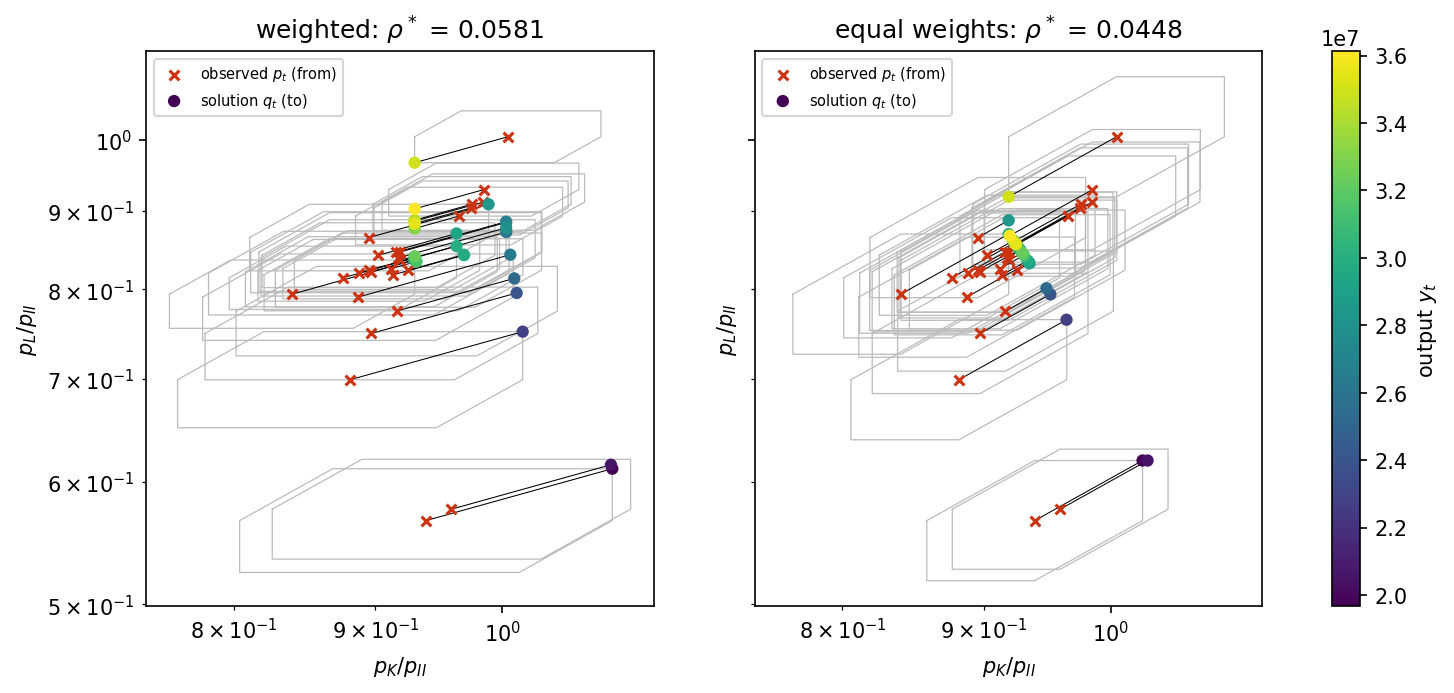
\includegraphics[width=\textwidth]{example_zono.png}
    \caption{Слева~--- решение при указанных штрафах, справа~--- при равных штрафах. Слева шаги не параллельны диагонали.}
\end{figure}

\subsection{Сдвиги с меняющимся направлением}

По теореме~\ref{thm:corners} решение периода $t$ лежит на пути $\theta\mapsto p_t\circ e^{\theta v_t}$, $v^i_t=1/\kappa^i_t+1/\kappa^0_t$. Направление сдвига точки $t$ в логарифмических координатах есть $v_t$. При штрафах вида $\kappa^i_t=\beta_i\tau_t$ имеем $v_t=v/\tau_t$ с общим $v$. Все сдвиги тогда параллельны, меняется только их допустимая длина. Так устроен пример выше.

Направления различаются, когда отношения штрафов зависят от периода. Пусть штраф цены капитала растёт со временем, а штрафы цен труда и промежуточных затрат постоянны:
\[
    \kappa^K_t=0.5+2.5\,\frac{t-t_0}{T-1},\qquad\kappa^L_t=\kappa^{II}_t=3.
\]
Тогда наклон $v^L_t/v^K_t$ растёт от $0.29$ в 1995 году до $1$ в 2020 году. Угол сдвига поворачивается от $16^\circ$ до $45^\circ$. В старые годы сдвиг почти горизонтален: двигается в основном цена капитала, в 1995 году $\Delta\ln(K/II)=+0.269$ при $\Delta\ln(L/II)=+0.077$. В 2020 году сдвиг идёт по диагонали: $\Delta\ln(K/II)=\Delta\ln(L/II)=-0.077$, то есть меняется только цена $II$. Для этих штрафов $\rho^*=0.11527$. Он больше, чем в примере выше, так как все штрафы здесь не меньше: в примере выше старые годы получали половинный штраф.

\begin{figure}[ht]
    \centering
    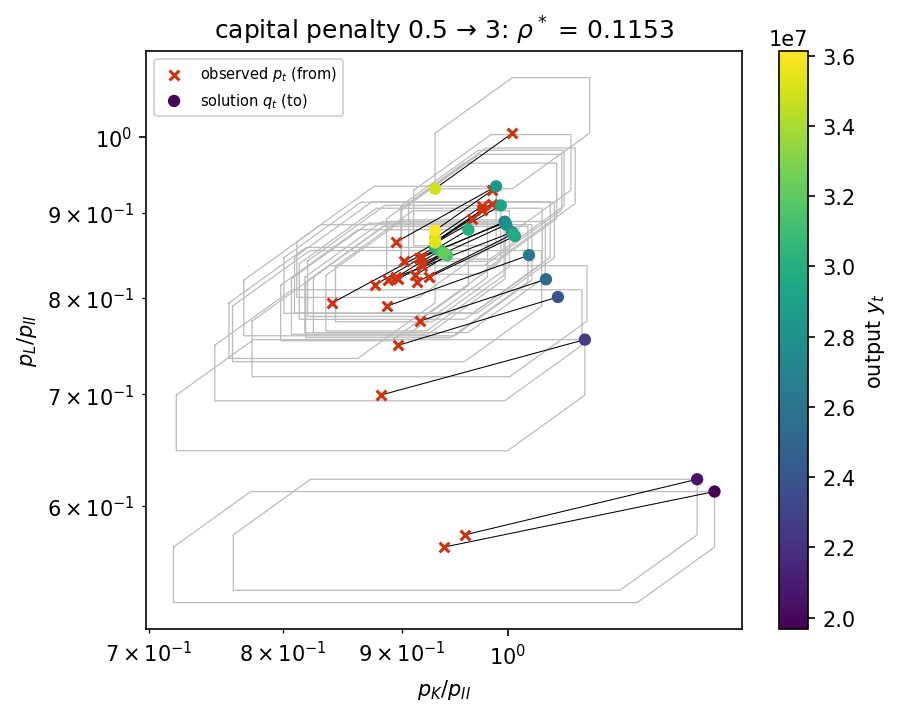
\includegraphics[width=0.62\textwidth]{example_rot.png}
    \caption{Штраф цены капитала растёт от $0.5$ до $3$, остальные штрафы равны $3$. Сдвиги старых лет (внизу) почти горизонтальны, сдвиги последних лет (вверху) идут вдоль диагонали.}
\end{figure}

\subsection{Сравнение оракулов при $d=2$ на реальных данных}

Данные BEA--BLS, $T=40$ (1977--2016), точки $(p_K/p_{II},p_L/p_{II})$, $y=\mathrm{GO\_Q}$, и EU KLEMS, США, $T=26$. Штрафы из таблицы выше. Бисекция с точностью $10^{-6}$, по $29$--$35$ обращений. Оба оракула дали один и тот же отрезок для $\rho^*$ во всех случаях. Безопасное округление ни разу не дало неопределённого ответа.
\begin{center}
\begin{tabular}{lrrr}
    \toprule
    данные & $\rho^*$ & поток, с & генерация столбцов, с \\
    \midrule
    EU KLEMS, США & 0.05807 & 3.1 & 10.3 \\
    BEA 1, Farms & 0.22882 & 51 & 35 \\
    BEA 6, Utilities & 0.19853 & 15 & 29 \\
    BEA 12, Machinery & 0.03886 & 207 & 41 \\
    BEA 15, Motor vehicles & 0.25271 & 10 & 13 \\
    BEA 24, Petroleum and coal & 0.47337 & 10 & 29 \\
    BEA 27, Wholesale trade & 0.05369 & 115 & 43 \\
    BEA 31, Water transportation & 0.04549 & 287 & 105 \\
    BEA 46, Rental and leasing & 0.02043 & 186 & 98 \\
    BEA 49, Misc.\ professional services & 0.02227 & 351 & 86 \\
    BEA 63, State and local & 0.15332 & 25 & 24 \\
    \bottomrule
\end{tabular}
\end{center}
Генерация столбцов быстрее в 7 случаях из 11, и именно там, где поток медленный, до 5 раз. Поток быстрее при большом $\rho^*$ и малом времени: на данных США и в отраслях 6, 15, 24.

\subsection{Синтетика при $d=2$}

Пять семейств A--E, $T=20,\dots,60$, одно обращение к оракулу при $\rho=0.05$: время потока и генерации столбцов. Семейства: случайные точки (A), точки около вогнутой дуги (B) и выпуклой дуги (C), точки целочисленной решётки (D), вогнутая дуга со случайными $y$ (E).

\begin{center}
\begin{tabular}{lrrrrr}
    \toprule
    семейство & $T=20$ & $T=30$ & $T=40$ & $T=50$ & $T=60$ \\
    \midrule
    A & \textbf{0.23} / 0.24 & 1.21 / 1.16 & 1.50 / 0.78 & 3.3 / 2.8 & 16.3 / 3.6 \\
    B & \textbf{0.32} / 0.58 & 1.48 / 1.19 & 4.5 / 2.6 & 10.9 / 2.9 & 23.3 / 9.3 \\
    C & 0.86 / 0.27 & 5.1 / 0.67 & 19.8 / 1.4 & 71.2 / 3.4 & 167.7 / 3.4 \\
    D & \textbf{0.07} / 0.18 & 0.87 / 0.42 & 2.3 / 1.5 & 5.2 / 2.2 & 13.2 / 4.5 \\
    E & 0.34 / 0.16 & 1.60 / 0.40 & 5.0 / 1.5 & 11.7 / 2.4 & 23.9 / 9.3 \\
    \bottomrule
\end{tabular}
\end{center}
В таблице время в секундах: поток / генерация столбцов. Жирным выделены случаи, где поток быстрее. Ответы совпали во всех 25 случаях. Поток быстрее только при $T=20$, на семействах A, B и D. Начиная с $T=30$ генерация столбцов быстрее во всех семействах. Худший случай для потока~--- выпуклая дуга, при $T=60$ разрыв около 50 раз.

Это только синтетика. Семейства подобраны вручную, и они не исчерпывают возможных трудных примеров. Пример, где поток быстрее при больших $T$, найти не удалось. Это не доказывает, что такого примера нет.

\subsection{Большие $d$}

Генерация столбцов с бисекцией по $\rho$ с точностью $10^{-5}$. Наборы данных: EU KLEMS, США, $d=3$ (цены K, L, II, нормирующая цена GO), Berndt--Wood, $d=4$, BEA--BLS, $d=4$ и $d=7$.
\begin{center}
\begin{tabular}{llrrr}
    \toprule
    данные & $d$, $T$ & $\rho^*$ & обращений & время, с \\
    \midrule
    EU KLEMS, США & 3, 26 & 0.03624 & 25 & 12 \\
    Berndt--Wood & 4, 25 & 0.01542 & 27 & 61 \\
    BEA 12, Machinery & 4, 40 & 0.05072 & 27 & 183 \\
    BEA 24, Petroleum and coal & 4, 40 & 0.15732 & 24 & 74 \\
    BEA 46, Rental and leasing & 4, 40 & 0.01598 & 24 & 183 \\
    BEA 6, Utilities & 4, 40 & 0.04333 & 27 & 282 \\
    BEA 24, Petroleum and coal & 7, 40 & 0.18847 & 28 & 782 \\
    BEA 12, 46, 6 & 7, 40 & \multicolumn{3}{l}{сбой вспомогательной задачи} \\
    \bottomrule
\end{tabular}
\end{center}
Штрафы: для EU KLEMS K 1, L 3, II 3, выпуск 4. Для Berndt--Wood K 1, L 3, E 2, M 3, выпуск 4. Для BEA при $d=4$ капитал 1, оба вида труда 3, II 3, выпуск 4. Для BEA при $d=7$ все виды капитала 1, оба вида труда 3, II 3. Множитель периода как выше. При $d\le4$ все случаи решены за минуты. При $d=7$ в трёх отраслях из четырёх вспомогательная задача 20 раз подряд вернула множества, не прошедшие точную проверку.

\section{Lean}

Библиотека \lean{PricePerturbation}, сборка \texttt{lake build PricePerturbation}, без \texttt{sorry}, только стандартные аксиомы.

\begin{center}
\begin{tabular}{p{0.38\textwidth}p{0.52\textwidth}}
    \toprule
    Утверждение & Lean \\
    \midrule
    лемма~\ref{lem:shape} (форма шара) & \lean{wdist_le_iff} \\
    следствие~\ref{cor:ball} & \lean{mem_wbox_of_wdist}, \lean{wdist_wpath_le} \\
    теорема~\ref{thm:corners}, (A)$\Leftrightarrow$(C) & \lean{wfeasible_iff_corners} \\
    теорема~\ref{thm:corners}, (A)$\Leftrightarrow$(B) & \lean{wfeasible_iff_path} \\
    (C)$\Rightarrow$(B), общий путь & \lean{path_of_corners} \\
    лемма~\ref{lem:signs} & \lean{witness_iff_homogeneous} \\
    лемма~\ref{lem:local} & \lean{eventually_exists_sign_eq} \\
    следствие~\ref{cor:local} & \lean{eventually_isWeakReachable_of} \\
    теорема~\ref{thm:least} (наименьший радиус) & \lean{least_wradius_breakpoint} \\
    радиусы по периодам (раздел~\ref{sec:profile}) & \lean{rfeasible_iff_corners}, \lean{rfeasible_iff_path} \\
    $\mathcal R$ замкнуто вверх и замкнуто & \lean{RFeasible.mono}, \lean{isClosed_setOf_rfeasible} \\
    минимальный по Парето элемент & \lean{exists_minimal_rfeasible} \\
    \bottomrule
\end{tabular}
\end{center}

Не формализованы: рациональность точек излома при равных штрафах, алгоритм и его сложность, сертификаты в коде.

\end{document}
